\chapter{Proces} \label{chap:proces}

For at sikre en struktureret udvikling af spillet, har vi udarbejdet efter en proces, der kombinere indledende planlægning med en initiativ og praktisk tilgang til kodning. Processen kan opdeles i kravspecifikation, systemdesign, implementering og integration. 

\textbf{Idegenerering og kravspecifikation}
\\Projekt forløbet startede ud med en grundig brainstorm-fase. Formålet var her først at definere de absolutte minimumskrav for at opfylde opgaveformuleringen. De den basale ramme var sat på plads, udvidede vi visionen for vores spil og opsatte egen krav til spillets funktionalitet. Denne tidlige fase var afgørende for at sikre at alle gruppemedlemmer havde en fælles forståelse for spillets mekanik, før kodnings processen gik i gang. 

\textbf{Systemarkitektur og opgave fordeling}
\\Inden selve programmeringsfasen påbegyndte, fastlage vi spillets overordnede struktur. Vi valgte en modulær opbygning, hvor koden blev opdelt i parrede .c- og .h-filer. Arkitekturen blev inddelt i fire hovedområder:

\vspace{-5pt}
\begin{itemize}
    \setlength{\itemsep}{0pt}
    \setlength{\parskip}{1pt}
    \setlength{\parsep}{0pt}
    \item Hardware: interaktion med joystick, LED og skærm
    \item Software infrastruktur: Underliggende systemer og kommunikationsproces
    \item Spille logik: beregning af fysik, kollision og bevægelses mønstre
    \item Spille design: visuel præsentation (ASCII-art) og menustruktur
\end{itemize}
\vspace{-5pt}

Opgaven blev fordelt ud fra gruppemedlemmernes individuelle styrker og interesser, hvilket sikrede at alle havde ejerskab over deres spesifike moduler. 

\textbf{Versionsstyring og værktøjer}
\\For at styrke effektiviteten har vi benyttet en række digitale værktøjer: 

\vspace{-5pt}
\begin{itemize}
    \setlength{\itemsep}{0pt}
    \setlength{\parskip}{1pt}
    \setlength{\parsep}{0pt}
    \item GitHub \& VS Code: Vi benyttede GitHub integreret direkte i VS Code. Dette gjorde det muligt løbende at "pushe" og "pulle" kode, hvilket minimerede risikoen for kodekonflikter og gjorde det nemt at gå tibage hvis en ny funktion introducerede fejl.
    \item ST-Link \& Putty: Debugging forgik via en serial forbindelse til Putty, som var med til at give mulighed for at monitorere variabler og programmets tilstand i real tid.
    \item Dokumentation: Rapportskrivning og journal føring skete løbende over Overleaf, mens overblikket over tidsplanen blev styret via et Gantt kort i Excel. 
\end{itemize}

\textbf{Integration og Debugging}
Projektforløbet var opdelt i to faser. Den første uge fungerede som en læring og forberedelsesfase, hvor fokus lå på at lære programmeringssproget C gennem en række undervisningsopgaver \ref{Journal}. Disse opgaver var nødvendige fundamentblokke til vores spil, herunder hardware interaktion, kontrol struktur, og forståelse af data typer.\\
I den anden uge skiftede vi fokus til selve projektet. Da vi allerede havde et godt fundament fra første uges opgaver, kunne vi hurtigt påbegynde integrationsfasen, hvor de isolerede kodebidder og logiske funktioner skulle samles til et sammenhængende spil. Dette var projektets mest kritiske fase, da vi her skulle sikre os at de forskellige moduler spillede sammen i realtid.
Vi lagde stor vægt på at definere klare input og output for vores funktioner således at de passede sammen på tværs af moduler. På trods af forsøget på en grundig planlægning opstod der udfordringer undervej, især omkring synkroniseringen af værdiger mellem forskellige logiske lag. 

\textbf{Kommunikation}
Det sociale og kommunikative fundament har været essentielt for at kunne gennemføre projekt inde for tidsgrænsen. Vi mødte op fysisk på skolen hver dag, hvilket gjorde det muligt at træffe hurtige valg og enriger ved problemer. Ved siden af det fysiske fremmøde havde vi også direkte adgang til alle gruppemedlemmer gennem beskeder, som blev brugt til hurtig opdatering og koordinering unden for skole tid. 

Denne strukturerede tilgang, hvor vi først byggede et solidt fundament i uge 1 og derefter arbejdede intensivt med integration i de følgende 2 uger, har gjort det muligt for os at gå fra de første øvelsesopgaver til et fuldt funktionelt spil med høj teknisk kompleksitet og tilhørende dokumentation.

For at visualisere denne udviklingsproces er der blevet udarbejdet et Gantt diagrammer. Det første diagram herunder \ref{fig:gantt_1}, illustrere vores oprindelige forventning til projektets gang. Det andet diagram \ref{fig:gantt_2} viser det faktiske forløb. Sammenligningen af disse to giver et klart billede af vores evne til at tilpasse os projektets reelle udfordringer undervejs.

\begin{figure}[H]
    \centering
    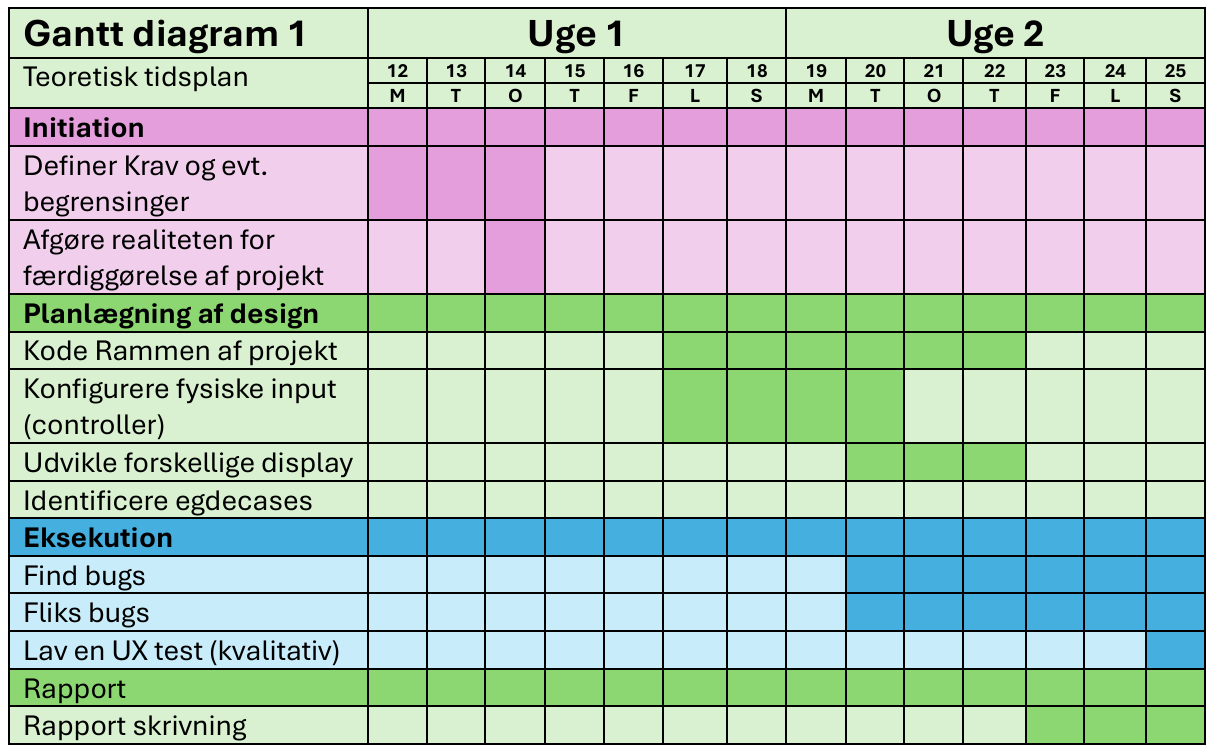
\includegraphics[width=0.81\textwidth]{Picturs/Diagrammer/Gantt1.png}
    \caption{Planlagt tidsplan udarbejdet ved projektstart}
    \label{fig:gantt_1}
\end{figure}
\vspace{-2em}
\begin{figure}[H]
    \centering
    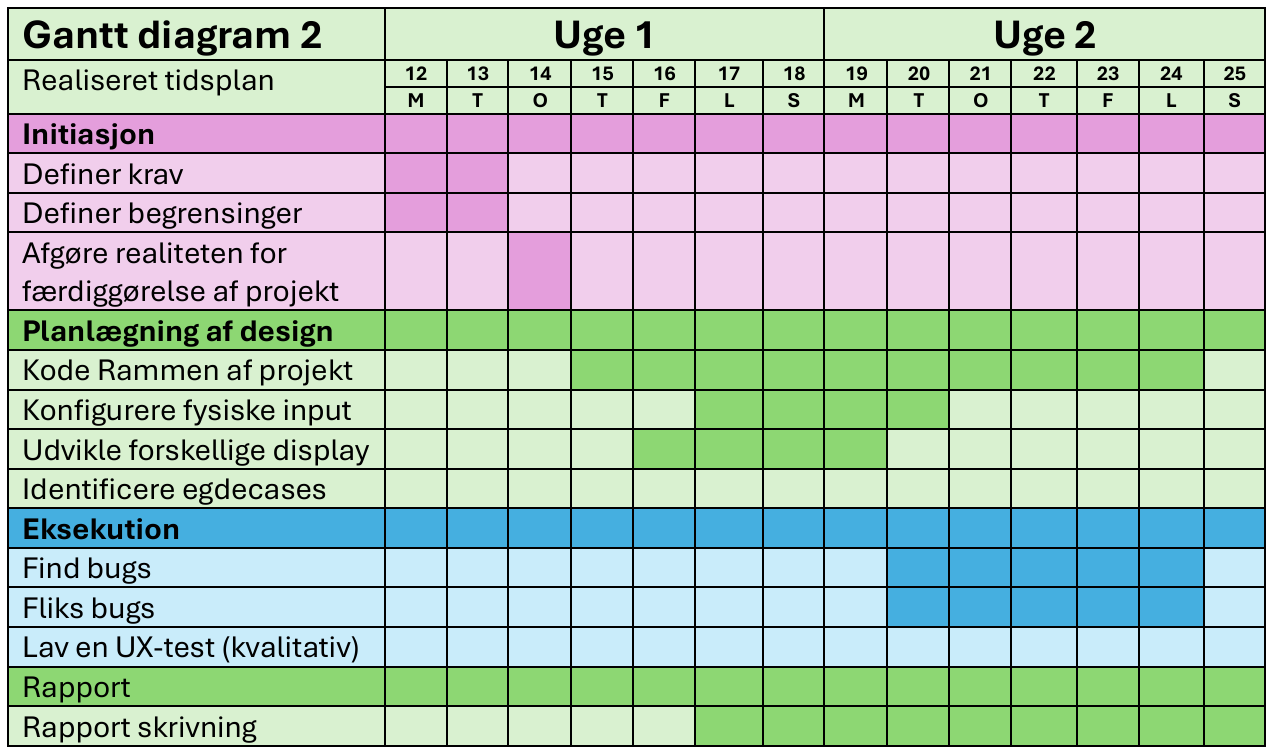
\includegraphics[width=0.81\textwidth]{Picturs/Diagrammer/Gantt2.png}
    \caption{Faktisk tidsforløb og eksekvering af projektfaser}
    \label{fig:gantt_2}
\end{figure}